\vspace{-1mm}
\section{Problem Statement}
%
\begin{wrapfigure}{r}{0.4\textwidth} %this figure will be at the right
    \vspace{-5mm}
    \centering
    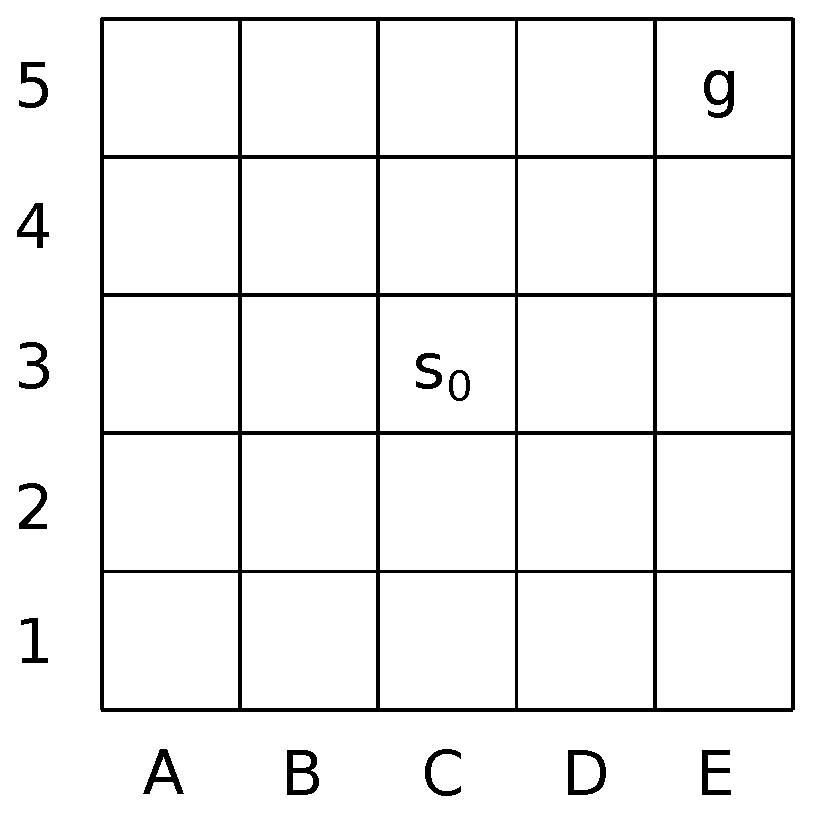
\includegraphics[width=0.25\textwidth]{./figures/drawing.eps}
    \caption{Schematic of the problem}
    \label{fig:schematic}
    \vspace{-5mm}
\end{wrapfigure}
%
% $5 \times 5$ bir satran\c{c} tahtas{\i} \"{u}st\"{u}ndeki karelerin yatayda A,
% B, C, D, E, dikeyde ise 1, 2, 3, 4, 5 \c{s}eklinde kodland{\i}\u{g}{\i}n{\i} ve
% C3 karesinde uzaktan kumandal{\i} bir robotunuz oldu\u{g}unu varsayal{\i}m.
% Robotun kumandas{\i}n{\i}n robotu yukar{\i}, a\c{s}a\u{g}{\i}, sola veya
% sa\u{g}a 1 kare hareket ettirecek \c{s}ekilde 4 tu\c{s}lu olarak
% tasarland{\i}\u{g}{\i}n{\i}, fakat haylaz karde\c{s}inizin kumandan{\i}n
% tu\c{s}lar{\i}n{\i}n yerlerini de\u{g}i\c{s}tirdi\u{g}ini d\"{u}\c{s}\"{u}nelim.
% Tu\c{s}lar{\i} bir kere kar{\i}\c{s}t{\i}r{\i}l{\i}p sabitlenen kumanda ile
% robotunuzu E5 noktas{\i}ndaki kareye g\"{o}t\"{u}rmek i\c{c}in basman{\i}z
% gereken minimum tu\c{s} say{\i}s{\i}n{\i}n beklenen de\u{g}eri ka\c{c}t{\i}r?


On a $5 \times 5$ chess board whose squares are coded by $A$, $B$, $C$, $D$, and
$E$ along the horizontal and by $1$, $2$, $3$, $4$, and $5$ along the vertical
direction, you have a remote-controlled robot on the square $C3$. The
remote-controller has $4$ buttons that can move the robot up, down, left, and
right by 1 square; however, your michievous sibling has tampered with the
placements of these buttons. Assuming that the buttons are fixed after having
shuffled once, what is the expected value of the number of times you need to
press the buttons in order to move the robot to the $E5$ square?